\documentclass[12pt, a4paper, oneside]{ctexart}
\usepackage{amsmath, amsthm, amssymb, graphicx}
\usepackage{hyperref}
\usepackage{listings}
\usepackage{xcolor}
\usepackage{color}
\usepackage{enumerate}
\usepackage{epstopdf}
\usepackage{float}
\usepackage{framed}
\usepackage[ruled,vlined]{algorithm2e}
\hypersetup{
    colorlinks=true,
    linkcolor=blue,
    filecolor=blue,      
    urlcolor=blue,
    citecolor=cyan,
}
\definecolor{dkgreen}{rgb}{0,0.6,0}
\definecolor{gray}{rgb}{0.5,0.5,0.5}
\definecolor{mauve}{rgb}{0.58,0,0.82}
\definecolor{shadecolor}{rgb}{0.5,0.5,0.5}
\lstset{ %
    language=Python,                % the language of the code
    basicstyle=\footnotesize,           % the size of the fonts that are used for the code
    numbers=left,                   % where to put the line-numbers
    %numberstyle=\tiny\color{gray},  % the style that is used for the line-numbers
    %stepnumber=2,                   % the step between two line-numbers. If it's 1, each line 
                            % will be numbered
    %numbersep=5pt,                  % how far the line-numbers are from the code
    %backgroundcolor=\color{blue},      % choose the background color. You must add \usepackage{color}
    showspaces=false,               % show spaces adding particular underscores
    %showstringspaces=false,         % underline spaces within strings
    showtabs=false,                 % show tabs within strings adding particular underscores
    frame=single,                   % adds a frame around the code
    rulecolor=\color{black},        % if not set, the frame-color may be changed on line-breaks within not-black text (e.g. commens (green here))
    tabsize=2,                      % sets default tabsize to 2 spaces
    captionpos=b,                   % sets the caption-position to bottom
    breaklines=true,                % sets automatic line breaking
    breakatwhitespace=false,        % sets if automatic breaks should only happen at whitespace
    % title=\lstname,                   % show the filename of files included with \lstinputlisting;
                            % also try caption instead of title
    keywordstyle=\color{blue},          % keyword style
    commentstyle=\color{dkgreen},       % comment style
    stringstyle=\color{mauve},         % string literal style
    escapeinside={\%*}{*)},            % if you want to add LaTeX within your code
    morekeywords={*,...}               % if you want to add more keywords to the set
}
\title{ICS\_Lab2\_Report}
\author{Xiaoma}
\date{\today}
\begin{document}
\maketitle
\section*{实验目的}
使用LC-3汇编命令实现
$$F(0) = F(1) = 1$$
$$F(N) = F(N-2) \% p + F(N-1) \% q \quad (2 \leq N \leq 1024)$$
$$p = 2^{k} \quad (2 \leq k \leq 10),10\leq q \leq 1024$$
\begin{itemize}
    \item p存储在内存位置\textbf{x3100}
    \item q存储在内存位置\textbf{x3101}
    \item N存储在内存位置\textbf{x3102}
    \item F(N)存储在内存位置\textbf{x3103}
\end{itemize}

\section*{实验原理}
对于求斐波那契数列的变式问题,通常情况下采用滑动窗口的方法。\\ \textbf{注意:本次实验计算公式与一般的斐波那契数列不同,$F(N-1),F(N-2)$
只有在求和的时候取余,而存储时不需要取余。}\\
按照该思想可以得到伪代码:

\begin{algorithm*}
    \caption{myFib}
    \label{alg:algorithm}
    \KwIn{p , q , N;}
    \KwOut{F(N) ;}
    \BlankLine
    num1 = 1;\\
    num2 = 1;\\
    N = N - 1;\\
    \While(){N > 0}{
        temp1 = num1;\\
        temp2 = num2;\\
        \While(){temp1 >= 0}{
            temp1 = temp1 - p;
        }
        temp1 = temp1 + p;\\
        \While(){temp2 >= 0}{
            temp2 = temp2 - q;
        }
        temp2 = temp2 + q;\\
        f = temp1 + temp2;\\
        num1 = num2;\\
        num2 = f;\\
        N = N -1;
    }
    \Return{f};
\end{algorithm*}

\section*{实验步骤}
\subsection*{LC-3指令集的限制}
若要实现上述伪代码,除了需要已知的8个变量,还需要2个变量来存储$p,q$的相反数,而LC-3只有8个寄存器,所以
需要对变量的数量进行压缩。
\begin{itemize}
    \item $F(N-2)$在完成本次计算以后将被移出窗口,即原存储$F(N-2)$的寄存器将存储$F(N-1)$。
    \item $F(N)$为两数取余之和
\end{itemize}
因此可以采用
\begin{itemize}
    \item $F(N-2)$与$F(N-2) \% p$共用一个变量
    \item 存储$F(N)$的变量首先存储$F(N-1)\% q$
    \item $F(N) = F(N) + F(N-2) \% p$
\end{itemize}
将所需寄存器的数量压缩至8个。

\subsection*{取余操作}
若需要用LC-3汇编命令实现取余操作,可将被除数不断减去除数,直至结果为负数,此时该负数与被除数相加
,得到的结果即为余数。
\subsection*{减法操作}
对于取余时需要的减法操作,采用与计算二进制数的相反数相同的方法,将原二进制数取反再加1。

\subsection*{计算斐波那契数列}
已知对于一个普通的斐波那契数列$F(N) = F(N-2) + F(N-1)$,假设有一个长度为3的窗口,每次窗口在数列上右移一位,
直至得到结果,即相当于每完成一次计算,后一个窗口存储前一个窗口的结果。

\subsection*{代码讲解}
\subsubsection*{初始化变量}
从内存中读取$p,q,N$ 3个变量,即$$R0 \leftarrow p, R1 \leftarrow q, R2 \leftarrow N$$
\begin{lstlisting}[name = code, firstnumber = 1]
    LD R0, x0FF
    LD R1, x0FF
    LD R2, x0FF
\end{lstlisting}
\subsubsection*{减法预处理}
已知取余操作要进行减法运算,故首先得到$p,q$的相反数,即$$R3 \leftarrow -p, R4 \leftarrow -q$$
\begin{lstlisting}[name = code, firstnumber = last]
    NOT R3, R0
    ADD R3, R3, x1
    NOT R4, R1
    ADD R4, R4, x1
\end{lstlisting}
\subsubsection*{取余操作}
分别求$F(N-2),F(N-1)$的余数,使用的变量考虑了LC-3寄存器的数量,即
$$R5 \leftarrow F(N-2) \% p, R7 \leftarrow F(N-1) \% q$$
\begin{lstlisting}[name = code, firstnumber = last]
    ADD R5, R5, R3 
    BRzp #-2
    ADD R5, R5, R0
    ADD R7, R6, #0
    ADD R7, R7, R4
    BRzp #-2
    ADD R7, R7, R1
\end{lstlisting}
\subsubsection*{求和}
求和得到$F(N)$,即
$$R7 \leftarrow F(N-2) \% + F(N-1) \% q$$
\begin{lstlisting}[name = code, firstnumber = last]
    ADD R7, R7, R5
\end{lstlisting}
\subsubsection*{滑动窗口}
得到计算结果后滑动窗口,准备下一个计算,即
$$R5 \leftarrow R6, R6 \leftarrow R7$$
\begin{lstlisting}[name = code, firstnumber = last]
    ADD R5, R6, #0
    ADD R6, R7, #0
\end{lstlisting}
\subsubsection*{存储结果}
在迭代结束后,将计算结过存储至x3103,即
$$R7 \rightarrow x3103$$
\begin{lstlisting}[name = code, firstnumber = last]
    ST R7, x0EC
\end{lstlisting}

\section*{如何提高循环效率}
观察$p$可以发现,$p$为2的整数次方,若用16位二进制数表示则只有一位为1,那么可以采用更简单的操作对$F(N-2)$进行取余。
\subsubsection*{更高效的取余操作}
若将$p$减去1以后将结果和$F(N-2)$进行与操作,则$F(N-2)$只有低位为1的部分被保留,即为$p$的余数。\\
\begin{lstlisting}
    ADD R3, R0, #-1
    AND R5, R5, R3 
\end{lstlisting}
\begin{figure}[H]
    \centering
    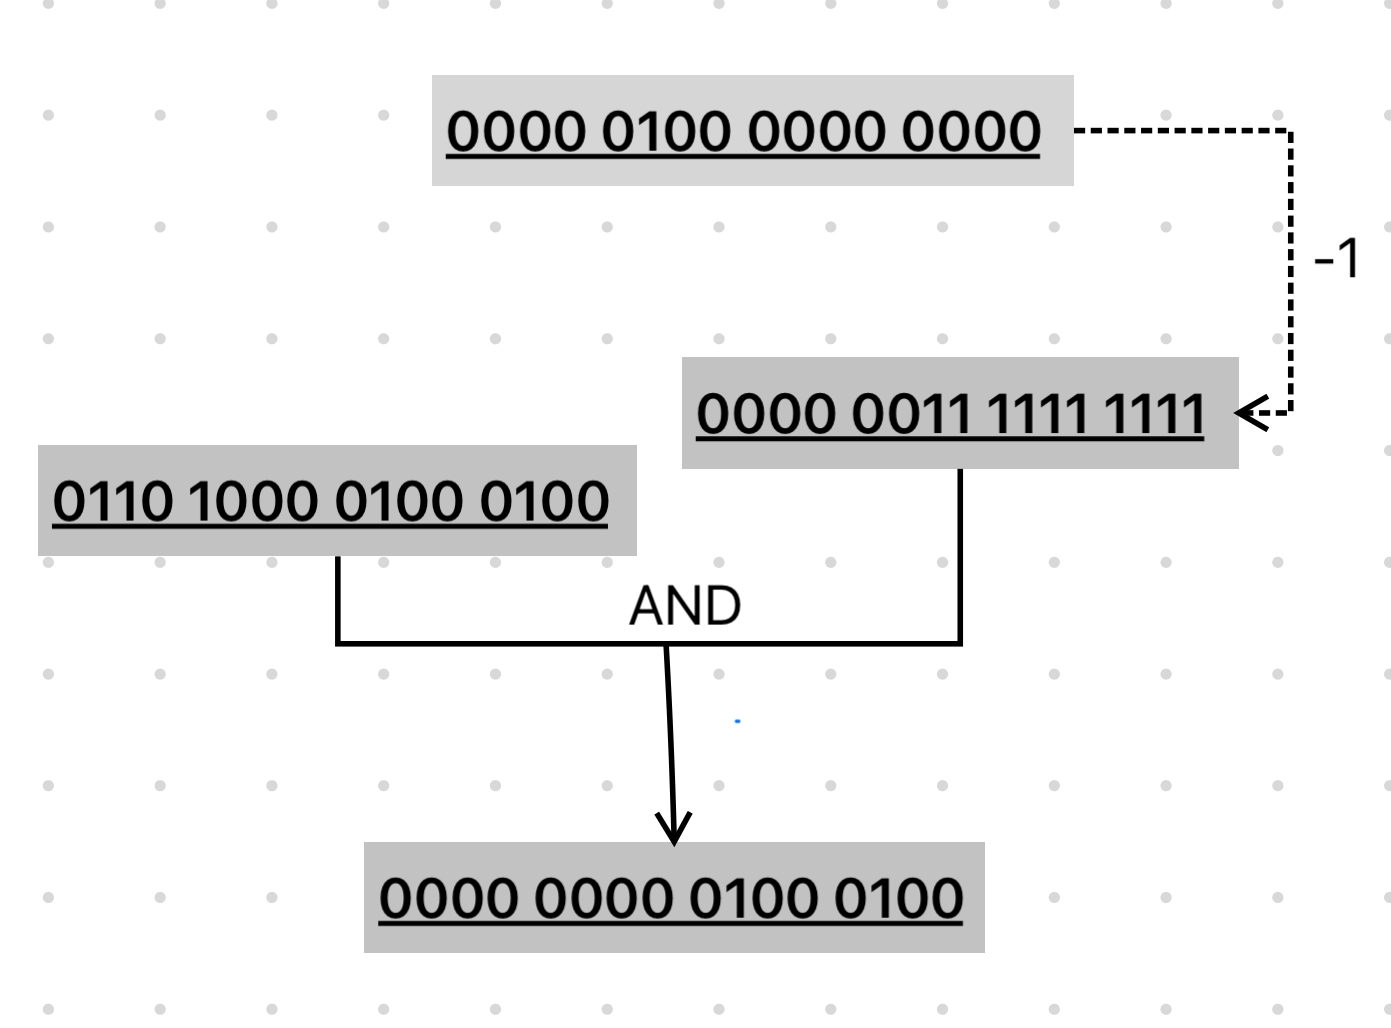
\includegraphics[scale=0.3]{quyu.png}
\end{figure}
\section*{实验结果}
\subsection*{未改进取余操作}
依次对实验文档给出的例子进行测试,结果如下:
\begin{figure}[H]
    \centering
    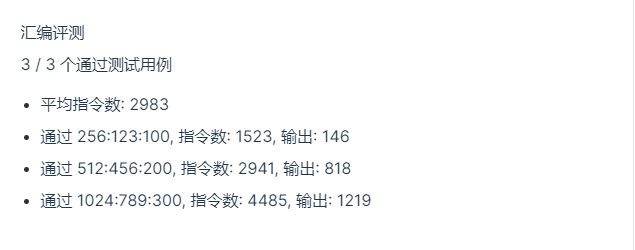
\includegraphics[scale=0.8]{Output1.png}
\end{figure}
自行编写了部分测试例子,结果如下:
\begin{figure}[H]
    \centering
    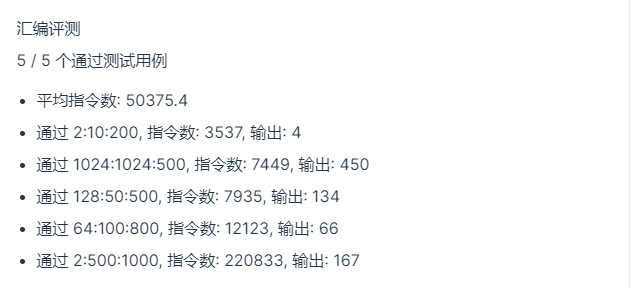
\includegraphics[scale=0.8]{Output2.png}
\end{figure}

\subsection*{改进取余操作}
依次对实验文档给出的例子进行测试,结果如下:
\begin{figure}[H]
    \centering
    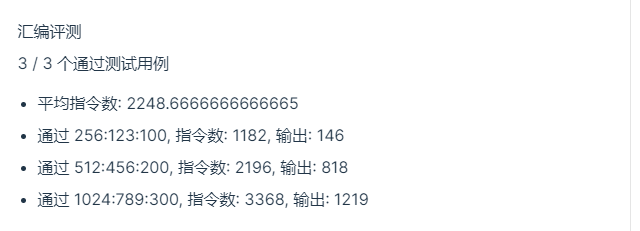
\includegraphics[scale=0.8]{Output4.png}
\end{figure}
自行编写了部分测试例子,结果如下:
\begin{figure}[H]
    \centering
    \includegraphics[scale=0.8]{Output5.png}
\end{figure}
可以发现改变取余操作大大提升了计算效率。
\end{document}


